\chapter{Benchmarking Tool}\label{chap:tool}
To facilitate future evaluations of the models on new datasets, we have
"wrapped" the raw code used for our evaluation into a \bld{graphical user
    interface (GUI) application}. We have decided to implement the GUI as a
\bld{web application}. This approach naturally solves the cross-platform (in
terms of operating systems) compatibility. Besides that, developing native
desktop applications can be very tedious; therefore, we have made this decision.
We believe that "running" a web interface is more natural today.

As we mentioned, the GUI (\bld{frontend}) is implemented as a web application
with a JavaScript framework. The application's logic (\bld{backend}) is
implemented separately in Python and is accessed by HTTP requests. In the
following sections, we describe the application's design and the implementation
details.

\section{Design}
The application's primary purpose is to train and evaluate selected models with
user-specified parameters on an arbitrary object detection dataset. We describe
the typical scenario of the user interactions with the application below:
\renewcommand{\theenumi}{\arabic{enumi}}
\begin{enumerate}
    \item The user uploads a new dataset or selects an old one. He can
          optionally define a split ratio by which the dataset will be split
          into training, test, and validation set.
    \item The user selects models to evaluate.
    \item The user sets selected models' parameters.
    \item The user initiates the training.
    \item The user then observes the results and eventually downloads the
          evaluation data.
\end{enumerate}
As we can see, the process can be split into a sequence of steps. Therefore, in
terms of the GUI design, we took inspiration from the layout of setup wizards
(see \myref{Figure}{fig:wizard}). At each step, only relevant information is
visible. The user can only go to the previous or next step (if the user provides
all the necessary information).

\begin{figure}[h]
    \centering
    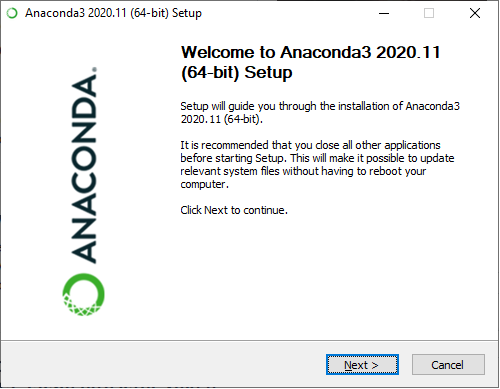
\includegraphics[width=0.65\linewidth]{Sources/Figures/anaconda.png}
    \caption{An example of a setup wizard.}
    \label{fig:wizard}
\end{figure}

The frontend communicates with the backend through the HTTP \bld{application
    programming interface (API)} composed of \bld{uniform resource identifier
    (URI)}
endpoints. The API will consist mainly GET and POST requests. For example, to
retrieve a list of datasets, we would send a GET request to a URI
of the form similar to \texttt{<api\_address>/datasets}. The POST requests will
be mainly used for setting up the training details and initiating the training
process. See \myref{Figure}{fig:tool_design} for an illustration of the communication.

\begin{figure}[h]
    \centering
    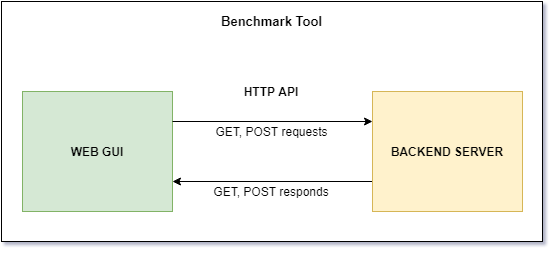
\includegraphics[width=0.85\linewidth]{Sources/Figures/tool_design.png}
    \caption{A diagram of bennchmarking tool's design.}
    \label{fig:tool_design}
\end{figure}

\section{Implementation}
The frontend is developed in \bld{Vue.js}. It is a JavaScript framework for
building interactive user interfaces. The interface is decomposed to many Vue
components that can communicate with each other and share the state. The
structure of the code is therefore more readable as it is written in a
semantical hierarchy of components. Each component is defined by its HTML
template that can be extended with JavaScript codes and Vue-specific special
constructs (such as \texttt{v-for} that can render elements of collections). See
demonstration in \myref{Listing}{code:vue}. The \texttt{v-for} is added to the
\texttt{<li>} element and renders it for each item in \texttt{items} JavaScript
array. The \texttt{\{\{ item.message \}\}} is used for text interpolation that
renders the JavaScript value as a HTML text.

\begin{lstlisting}[language=HTML, caption=Vue.js template example]
<ul>
    <li v-for="item in items">
        {{ item.message }}
    </li>
</ul>
\end{lstlisting}
\label{code:vue}

It is common to use CSS frameworks when implementing a non-trivial graphical
interface. They allow us to use predefined components, a grid-based positioning
system, or a predefined set of typographic utilities. We have therefore used the
\bld{Material Design Framework Vuetify}. Fortunately, the framework already
includes a "stepper" component that corresponds to the proposed design in the
previous section. The component progresses vertically from top to bottom. The
current progress is visible on the left side of the component. Similar to the
setup wizards, the user can only move one step back or one step forward in each
step by clicking on the buttons in the bottom left corner of each step's body.
The implementation can be seen in \myref{Figure}{fig:datasets_selection}.

\begin{figure}[h]
    \centering
    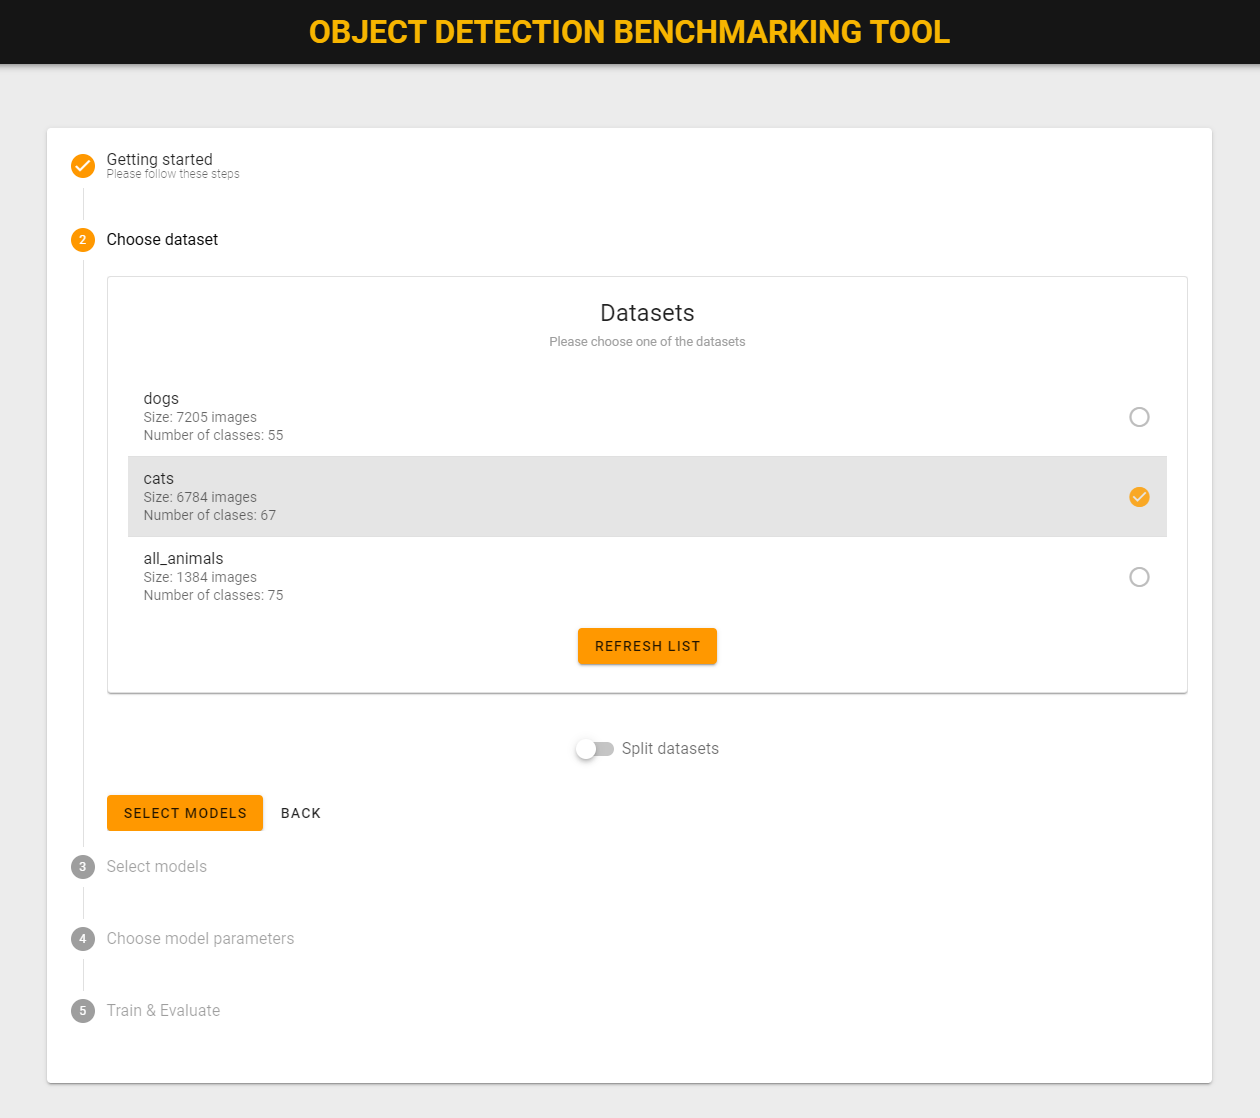
\includegraphics[width=0.85\linewidth]{Sources/Figures/datasets_selection.png}
    \caption{Implementation of the stepper layout.}
    \label{fig:datasets_selection}
\end{figure}

The first step is introductory. It describes the required dataset folder
structure and formats. On top of that, it shows the destination folder where the
user should upload the dataset. The next step serves for the selection of the
available datasets. It automatically lists all datasets that are correctly
uploaded. The datasets that are detected but are of the wrong format or miss
some necessary details cannot be chosen. Besides that, an appropriate warning
is shown to the user. All available datasets are shown in a list with additional
information such as the size of the dataset or the number of classes it consists
of (see \myref{Figure}{fig:datasets_selection}). By clicking on one of the list's
item, a corresponding dataset is chosen. If a file containing all the
annotations is present in the selected dataset's folder, the user can also
choose a split ratio by which the dataset is automatically divided. After
selecting the dataset, the user has to choose the models to be evaluated. The
list is similar to the datasets list, with the exception that the user can
choose multiple items from the list. The next step is to choose the values of
the parameters of each model.

\begin{figure}[ht]
    \centering
    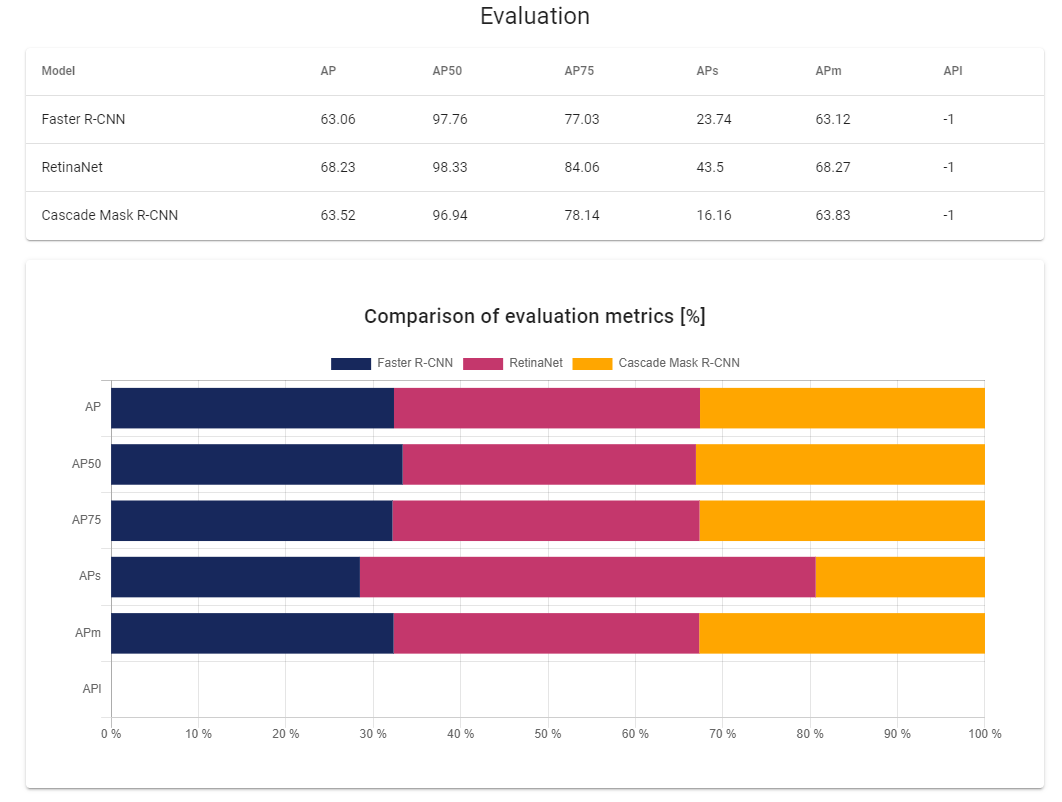
\includegraphics[width=1.1\linewidth]{Sources/Figures/eval_table_plot.png}
    \caption{Evaluation step in benchmarking tool.}
    \label{fig:evaluation-step}
\end{figure}

Finally, the last step recapitulates the chosen models and selected parameters.
The user initiates the training by clicking on a "Start training" button. Since
the training process can be long, the user should have feedback on the training
progress. We therefore display the console's output by polling the training logs
from the backend. After the training finishes, the models are immediately
evaluated. First, the table of AP metrics is shown. Each column can be sorted in
both descending and ascending order by clicking on the metric's name. Next, we
visualize the metrics in a stacked bar chart to highlight the differences in the
values (see \myref{Figure}{fig:evaluation-step}). The last evaluation component of
the benchmarking tool is the option to view the prediction results on a random
test image for each trained model (see \myref{Figure}{fig:random-inference}). The
user can choose between predictions of trained models and set the score
threshold (predictions with the score above the threshold are counted as
true positives).

\begin{figure}[ht]
    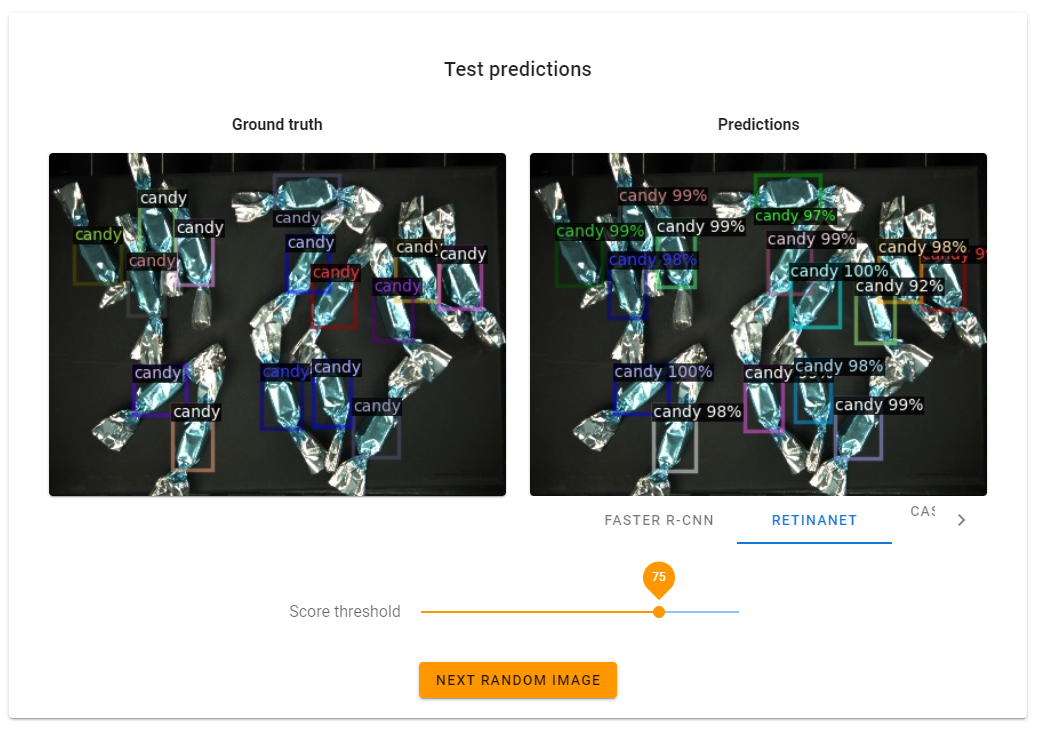
\includegraphics[width=\linewidth]{Sources/Figures/eval_random_image_.png}
    \caption{Predictions on a random image in benchmarking tool.}
    \label{fig:random-inference}
\end{figure}

The trained weights can be downloaded in the PyTorch \texttt{.pth} format. The
format is based on Python's object serialization module \texttt{pickle}. The
module is used for converting Python object hierarchies to byte stream that can
be later deserialized or "unpickled".

As we mentioned in the beginning of this chapter, the backend is implemented in
Python. Since the Detectron2 framework is based on Python, it was a natural
choice to preserve the technology. The HTTP API is implemented with
\bld{FastAPI} library that enables a straightforward creation of the API
endpoints based on standard Python type hints. That means the instances of some
custom defined Python data models can be automatically validated and converted
e.g. to JSON.
\newpage
\begin{lstlisting}[language=python, caption=Simplified FastAPI example]
    from fastapi import FastAPI

    app = FastAPI()

    @app.get("/datasets")
    def read_datasets():
        return ["candies", "medical", "metal"]
\end{lstlisting}
\label{code:fastapi}

See \myref{Listing}{code:fastapi} for a simplified FastAPI usage.
Sending a GET request to the \texttt{/datasets} endpoint would return a JSON
array \texttt{["candies", "medical", "metal"]}. We can define POST endpoints in
similar manner. The main logic is implemented in the \texttt{Benchmark} class.
The instance of the class preserves the application's state and handles most of
the requests sent by the frontend.

